\subsection{问题4}

\subsubsection{精度与稳定性分析}
问题4要求分析问题1中参数标定的精度和稳定性,下面逐一进行讨论。

首先考虑求解接收器间距$l$时使用的回归方法的精度。我们可以认为由于外界干扰以及机器自身的内禀影响,测量得到的值 $L_m$ 与真实值 $\hat L_m$ 之间有如下关系:

\begin{equation}
	L_m = \hat L_m + \sigma\varepsilon_m\text{, } \varepsilon_m \sim \mathcal N(0, 1)
	\label{equ:4_relation}
\end{equation}

并且$\varepsilon_0, \varepsilon_1, \cdots, \varepsilon_n$之间相互独立。

那么对于公式$\ref{equ:1_reg}$中右侧量$L_0^2-L_m^2$可以计算其方差:

\begin{equation}
	\begin{aligned}
		\var[L_0^2-L_m^2] &= \var[(\hat L_0 + \sigma\varepsilon_0)^2] + \var[(\hat L_m - \sigma\varepsilon_m)^2] \\
		&\leq \var[2\sigma\varepsilon_0] + \var[\sigma^2\varepsilon_0^2] + \var[2\sigma\varepsilon_m] + \var[\sigma^2\varepsilon_m^2] \\
		&= 8\sigma^2 + 4\sigma^4
	\end{aligned}
	\label{equ:4_reg_var}
\end{equation}

如果利用$l_0, \cdots, l_n$共$n + 1$条直线来计算接收器间隔$l$,将公式$\ref{equ:1_reg}$中的回归方程记为$Ax=L$,其中$L=\frac{1}{4}(L_0^2-L_1^2, \cdots, L_0^2 - L_n^2)^T$,$x = ((D_0-R)l, l^2)^T$,并且$x = (A^TA)^{-1}A^TL$,计算可得

\begin{equation}
	(A^TA)^{-1} =
	\begin{bmatrix}
		\frac{9}{2 \left(n^2+n-2\right)} & -\frac{6 (2 n+1)}{n (n+1) \left(n^2+n-2\right)} \\
		-\frac{6 (2 n+1)}{n (n+1) \left(n^2+n-2\right)} & \frac{36}{n (n+1) \left(n^2+n-2\right)} \\
	\end{bmatrix}
	\label{equ:4_ATA_reg}
\end{equation}

为了符号简便,将矩阵\ref{equ:4_ATA_reg}第二行记为$(a_{21}, a_{22})$,可以得到

\begin{equation}
	\begin{aligned}
		\var[l^2] &\leq \var[a_{21}\sum_{i=1}^n 2iL_i] + \var[a_{22} \sum_{i=1}^ni^2L_i] \\
		&\leq \frac{2\sigma^2 + \sigma^4}{4}\left[ a_{21}^2 P_3(n) + a_{22}^2 P_5(n) \right] \\
		&=\frac{2\sigma^2 + \sigma^4}{Q_3(n)}
\end{aligned}
	\label{equ:4_var_finite}
\end{equation}

其中 $P_3(n), P_5(n)$ 分别是关于$n$的$3$次多项式和$5$次多项式,$Q_3(n)$是关于$n$的$3$次多项式。因此,我们知道$\var[l^2]$和$n$至少为立方反比关系。

\begin{figure}[htbp]
  \centering

  \begin{subfigure}[b]{0.3\textwidth}
    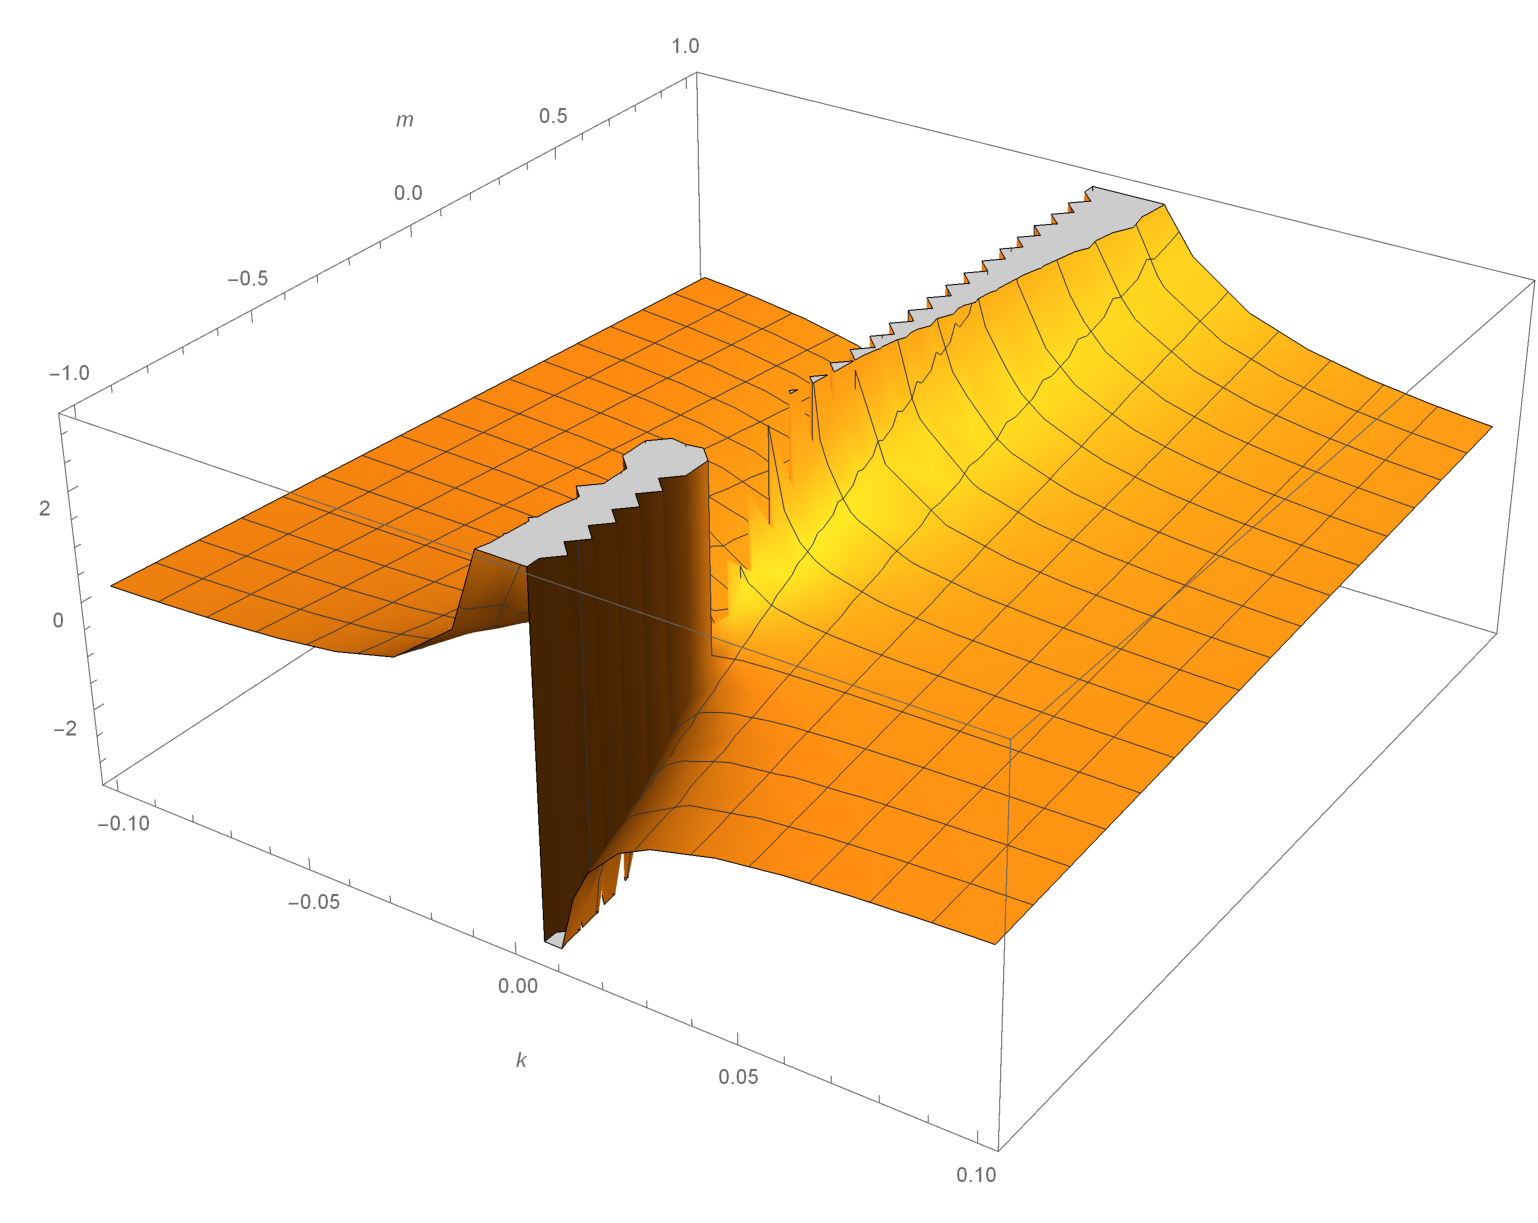
\includegraphics[width=\linewidth]{4_slope_fault_2.pdf}
    \caption{$\displaystyle \frac{\partial k}{\partial L_0}, |k| \leq 0.1 $}
    \label{fig:4_slope_fault:1}
  \end{subfigure}%
  \hfill
  \begin{subfigure}[b]{0.3\textwidth}
    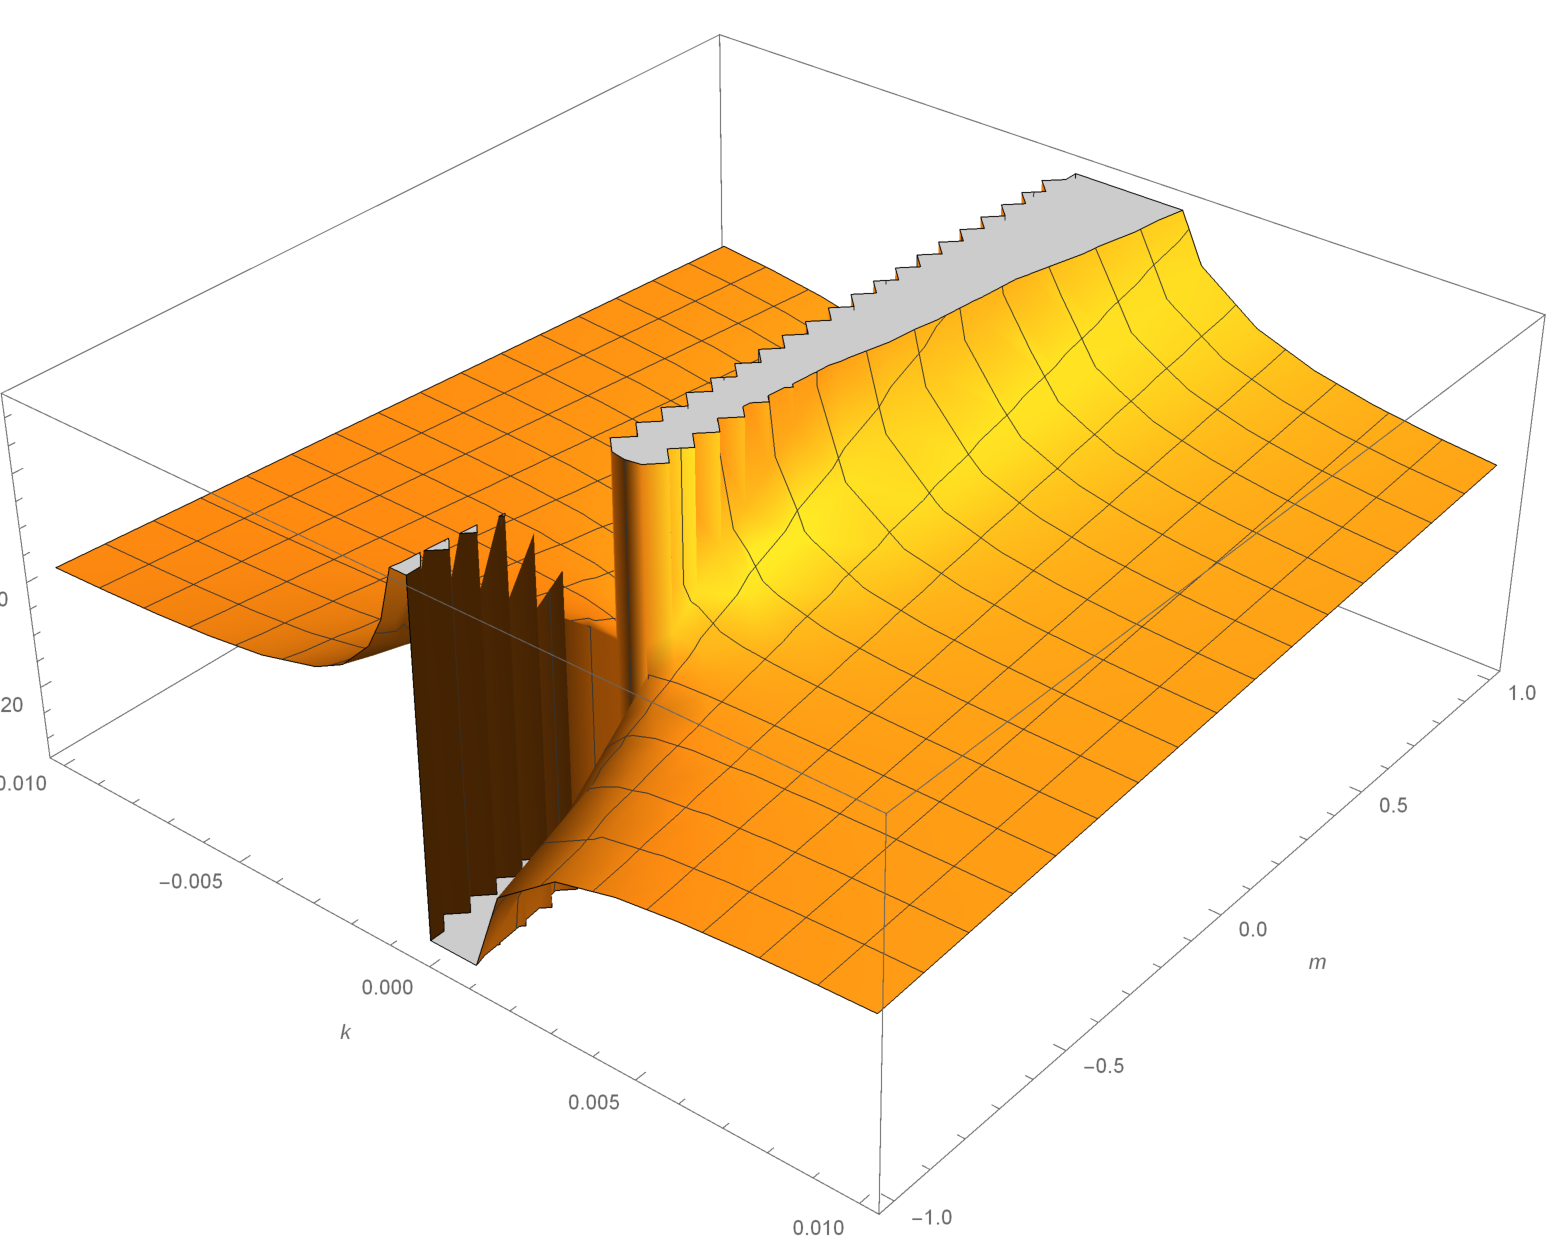
\includegraphics[width=\linewidth]{4_slope_fault.pdf}
    \caption{$\displaystyle \frac{\partial k}{\partial L_0}, |k| \leq 0.01 $}
    \label{fig:4_slope_fault:2}
  \end{subfigure}%
  \hfill
  \begin{subfigure}[b]{0.3\textwidth}
    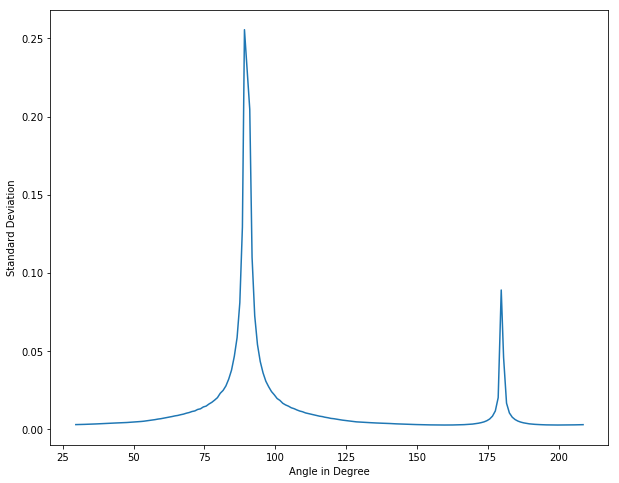
\includegraphics[width=\linewidth]{4_std_err_degree.png}
    \caption{计算得到$\omega$的标准差}
    \label{fig:4_std_err_degree}
  \end{subfigure}

  \caption{图\subref{fig:4_slope_fault:1}与图\subref{fig:4_slope_fault:2}是当$k$在不同范围内变化时,可以观察到当$k \to 0$时,$\displaystyle \frac{\partial k}{\partial L_0} \to \infty$;由图\subref{fig:4_std_err_degree}可见当椭圆轴与射线接近平行时计算得到的$\omega$标准差有突增}
  \label{fig:4_analysis}
\end{figure} 

对于角度的计算,我们是通过方程组\ref{equ:1_degree_full}中联立相邻两个方程再取平均来完成的。如图\ref{fig:4_std_err_degree},在投影线和椭圆的轴接近平行时标准差较大,下面将会分析该现象发生的原因。

首先将方程\ref{equ:1_degree_full}中的弦长写成关于$m_0$和$\omega$的函数$G_i(\omega, m_0) = G_i(\arctan k, m_0)$。为了方便,我们不妨设联立的两个方程为

\begin{equation}
	\left\{
		\begin{aligned}
			G_0(\omega, m_0) &= L_0 \\
			G_i(\omega, m_0) &= L_i
		\end{aligned}
	\right.
	\label{equ:5_length_eq2}
\end{equation}

根据反函数定理,如果$\partial (L_0, L_i) / \partial (\omega, m_0)$存在,那么

\begin{equation}
	\frac{\partial(\omega, m_0)}{\partial(L_0, L_i)}
	= \left[\frac{\partial(L_0, L_i)}{\partial(\omega, m_0)}\right]^{-1}
	= \left[\frac{\partial(L_0, L_i)}{\partial(k, m_0)}\cdot \frac{\partial(k, m_0)}{\partial(\omega, m_0)}\right]^{-1}
	\label{equ:5_inv_partial}
\end{equation}

记 $\displaystyle J_\omega(\omega, m_0) = \frac{\partial(L_0, L_i)}{\partial(\omega, m_0)}$,$\displaystyle J_k(k, m_0) = \frac{\partial(L_0, L_i)}{\partial(k, m_0)}$,从公式\ref{equ:1_degree_full}可以看出$J_\omega(\omega, m_0)$的各个元素在原点附近都是连续可微的。并且计算后可得

\begin{equation}
	J_\omega(0, m_0) = J_k(0, m_0) = \begin{bmatrix}
		0 & -\frac{2 a m_0}{b \sqrt{b^2 - m_0^2}} \\
		0 & -\frac{2 a (i l+m_0)}{b \sqrt{b^2 - (i l+m_0)^2}} \\
	\end{bmatrix},
	\label{equ:5_jacob_k0}
\end{equation}

我们可以设

\begin{equation}
	J_\omega(\omega, m_0) = \begin{bmatrix}
		A(\omega, m_0) & B(\omega, m_0) \\
		C(\omega, m_0) & D(\omega, m_0)
	\end{bmatrix}
	\label{equ:5_j_omega}
\end{equation}

这样当 $\det J_\omega$ 非零时,该矩阵可逆并且

\begin{equation}
	J_\omega^{-1}(\omega, m_0) = \frac{1}{\det J_\omega(\omega, m_0)}
	\begin{bmatrix}
		D(\omega, m_0) & -B(\omega, m_0) \\
		-C(\omega, m_0) & A(\omega, m_0)
	\end{bmatrix}
	\label{equ:5_j_omega_inv}
\end{equation}

由公式\ref{equ:5_jacob_k0}以及$A, B, C, D$的连续性可知,当$\omega \to 0$时,$A \to 0$且$C \to 0$。而此时,根据$m_0$的几何意义可知$|m_0| < b$,不妨认为在选取数据时忽略距离椭圆边界最近的两条直线,那么$B, D$在原点附近有界。因此可以得到

\begin{equation}
	\det J_\omega(\omega, m_0) = AD - BC \to 0
	\label{equ:5_det_to_0}
\end{equation}

那么就有

\begin{equation}
	\frac{\partial \omega}{\partial L_0} = \frac{D(\omega, m_0)}{\det J_\omega(\omega, m_0)}  \to \infty,\quad\quad
	\frac{\partial \omega}{\partial L_i} = \frac{D(\omega, m_0)}{\det J_\omega(\omega, m_0)}  \to \infty
	\label{equ:5_partial_to_inf}
\end{equation}

这样,根据\ref{equ:4_relation},在存在一个白噪声$\varepsilon\sim\mathcal N(0, \sigma^2)$的情况下,当投影线与椭圆的轴平行的时候所求得的$\omega$的方差将会过大。相应地,$\theta$的方差也变大。

综上,我们得到如下的分析结果:
\begin{principle}
\label{prcp:l_n}
回归得到的$l$精确程度与穿过圆区域的射线数目成正相关
\end{principle}

\begin{principle}
\label{prcp:omega}
当射线与椭圆的轴接近平行时,随机噪声的存在将使$\theta$的求解结果变得不稳定
\end{principle}

最后,由于旋转中心的坐标可$C(X_0,Y_0)$完全由上述求得的$l$与$\theta$所确定,故其精度与稳定性受到上述两个因素的共同制约。


\subsubsection{模板设计与模型修正}

下面提出一个简单的模板设计来减轻上述问题对标定产生的影响。

对于定律\ref{prcp:l_n}的结论,已知增大穿过圆的射线条数$n$能够增加$l$的精确程度。由于接收器间隔是一定的,故应当增大模型上圆形区域的尺寸。对于定律\ref{prcp:omega}的结论,我们应当尽量避开射线与椭圆轴平行的角度(至多有三个位置),故可以每次扫描后将椭圆模板绕其中心旋转一定角度,重复多次这样的操作,就能获取充分多的数据避开“坏”的角度。

本参数标定模型的模板包含一至多个半径不同的圆与一个椭圆,并且其吸收率均相同(如1.0000)。在每次扫描时均只使用其中的一个,避免扫描条带出现重叠现象影响数据的处理。

对于接收器间距$l$的计算,可选取半径较大的圆(可以考虑直径为托盘宽度的$2/3$),圆心与托盘中心重合,再利用第\ref{sec:1_calc_l}节提出的回归算法计算$l$。如果认为方差过大或者精度不足可以改变圆的位置或半径多次计算并且取平均值。$l$值的计算与圆心所处的位置无关。

对于探测系统相对于初始状态旋转角度$\theta$的计算,选取中心位于托盘中心的,长轴长约为托盘宽度$2/3$且与x轴平行的椭圆。设$n$为总共的扫描次数(一般推荐取5左右),则每次椭圆旋转的角度应为$\pi/n$。假设第$i$扫描得到的第$j$个旋转角度的估计值为$\theta_{i,j}$,数据的标准差为$s_{i,j}$,且$\alpha_i = \argmin_j s_{i,j}$,则最后确定的旋转角度$\theta_i$为$\theta_{i, \alpha_i}$。 